\iffalse
\documentclass[12pt]{article}
\usepackage{graphicx}
\usepackage{amsmath}   % for having text in math mode

%Following 2 lines were added to remove the blank page at the beginning
\usepackage{atbegshi}% http://ctan.org/pkg/atbegshi
\AtBeginDocument{\AtBeginShipoutNext{\AtBeginShipoutDiscard}}
%

\begin{document}

\begin{center}
\title{\textbf{Area of a Traingle}}
\date{\vspace{-5ex}} %Not to print date automatically
\maketitle
\end{center}

\setcounter{page}{1}



\section{10$^{th}$ Maths - Chapter 7}

All problems are from Exercise 7.3

\fi
%\begin{enumerate}[label=\thechapter.\arabic*,ref=\thechapter.\theenumi]
\begin{enumerate}[label=\thesection.\arabic*,ref=\thesection.\theenumi]
\numberwithin{equation}{enumi}
\numberwithin{figure}{enumi}
\numberwithin{table}{enumi}
\item Find the area of the triangle whose vertices are 
\begin{enumerate}
\item $(2, 3), (–1, 0), (2, – 4)$
\item $(–5, –1), (3, –5), (5, 2)$ 
\end{enumerate}
		\label{10/7/3/1}
\solution
		\iffalse
\documentclass[12pt]{article}
\usepackage{graphicx}
%\documentclass[journal,12pt,twocolumn]{IEEEtran}
\usepackage[none]{hyphenat}
\usepackage{graphicx}
\usepackage{listings}
\usepackage[english]{babel}
\usepackage{graphicx}
\usepackage{caption} 
\usepackage{hyperref}
\usepackage{booktabs}
\usepackage{array}
\usepackage{amsmath}   % for having text in math mode

%Following 2 lines were added to remove the blank page at the beginning
\usepackage{atbegshi}% http://ctan.org/pkg/atbegshi
\AtBeginDocument{\AtBeginShipoutNext{\AtBeginShipoutDiscard}}
%


%New macro definitions
\newcommand{\mydet}[1]{\ensuremath{\begin{vmatrix}#1\end{vmatrix}}}
\providecommand{\brak}[1]{\ensuremath{\left(#1\right)}}
\providecommand{\norm}[1]{\left\lVert#1\right\rVert}
\newcommand{\solution}{\noindent \textbf{Solution: }}
\newcommand{\myvec}[1]{\ensuremath{\begin{pmatrix}#1\end{pmatrix}}}
\let\vec\mathbf

\begin{document}

\begin{center}
\title{\textbf{Area of a Traingle}}
\date{\vspace{-5ex}} %Not to print date automatically
\maketitle
\end{center}

\setcounter{page}{1}



\section{10$^{th}$ Maths - Chapter 7}

This is Problem-1 from Exercise 7.3

\begin{enumerate}
\item Find the area of the triangle whose vertices are :
	\fi
\begin{enumerate}
\item 
In this case, the area  is given by  
  \label{prop:10/7/3/1area2d}
  \begin{align}
    \label{eq:10/7/3/1area2d}
	\frac{1}{2}\norm{\brak{\vec{A}-\vec{B}} \times \brak{\vec{A}-\vec{C}}} \\
  \end{align}
  Since
  \begin{align}
	 \vec{A}-\vec{B} =  \myvec{
  2 \\
  3 \\
 } - \myvec{
  -1 \\
  0 \\
 } = \myvec{
 3 \\
 3 \\
 }
 \\
 \vec{A}-\vec{C} =  \myvec{
  2 \\
  3 \\
 } - \myvec{
  2 \\
  -4 \\
 } = \myvec{
 0 \\
 7 \\
 }
 \end{align}
 the desired area is given by 
 \iffalse
The value of the cross product of two vectors is given by
\begin{align}
  \label{eq:10/7/3/1det2d}
  \mydet{\vec{M}} &= \mydet{\vec{A} & \vec{B}} 
  \\
  &= \mydet{a_1 & b_1\\a_2 & b_2} = a_1b_2 - a_2 b_1
\end{align}

		Therefore, \eqref{eq:10/7/3/1area2d} equals \\
		\fi
\begin{align}
	\frac{1}{2}\mydet{3 & 0\\3 & 7}  
	&=	\frac{21}{2}
\end{align}
\iffalse
\begin{figure}[!h]
	\begin{center}
		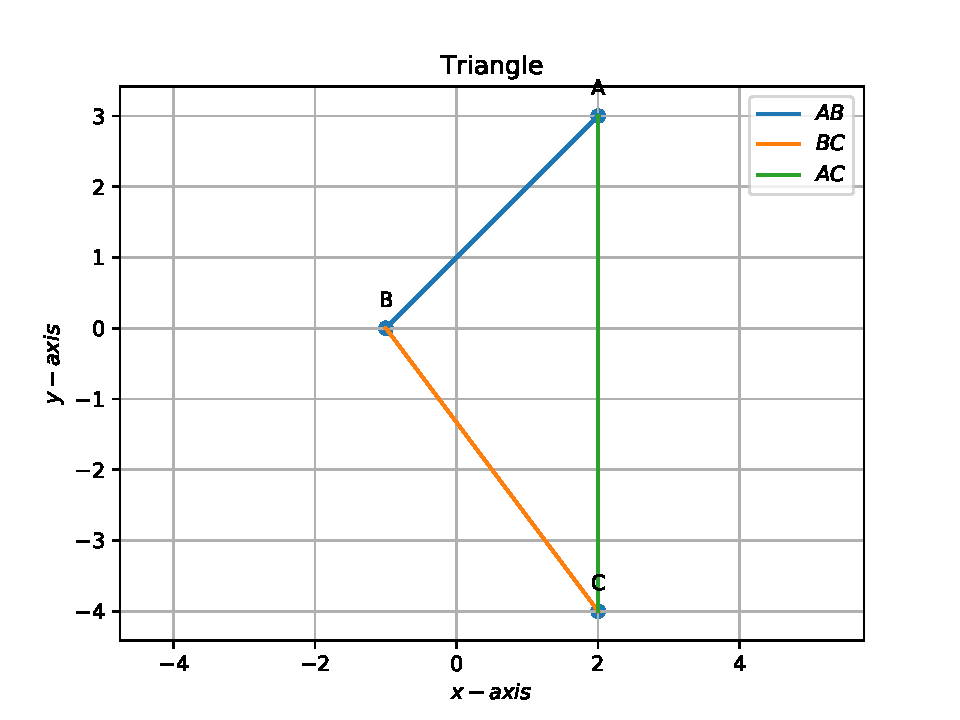
\includegraphics[width=\columnwidth]{./figs/problem1a.pdf}
	\end{center}
\caption{}
\label{fig:Fig1}
\end{figure}
\fi

\item In this case, 
	\iffalse
\solution The area of the triangle with vertices $\vec{A}, \vec{B}, \vec{C}$ is given by  
  \label{prop:10/7/3/1area2e}
  \begin{align}
    \label{eq:10/7/3/1area2e}
	\frac{1}{2}\norm{\brak{\vec{A}-\vec{B}} \times \brak{\vec{A}-\vec{C}}} \\
	\fi
  \begin{align}
	 \vec{A}-\vec{B} =  \myvec{
  -5 \\
  -1 \\
 } - \myvec{
  3 \\
  -5 \\
 } = \myvec{
 -8 \\
 4 \\
 }
 \\
 \vec{A}-\vec{C} =  \myvec{
  -5 \\
  -1 \\
 } - \myvec{
  5 \\
  2 \\
 } = \myvec{
 -10 \\
 -3 \\
 }
 \\
	  \implies
\text{Area} =	\frac{1}{2}\mydet{-8 & -10\\4 & -3}  
	=  32 
\end{align}
\iffalse
\begin{figure}[!h]
	\begin{center}
		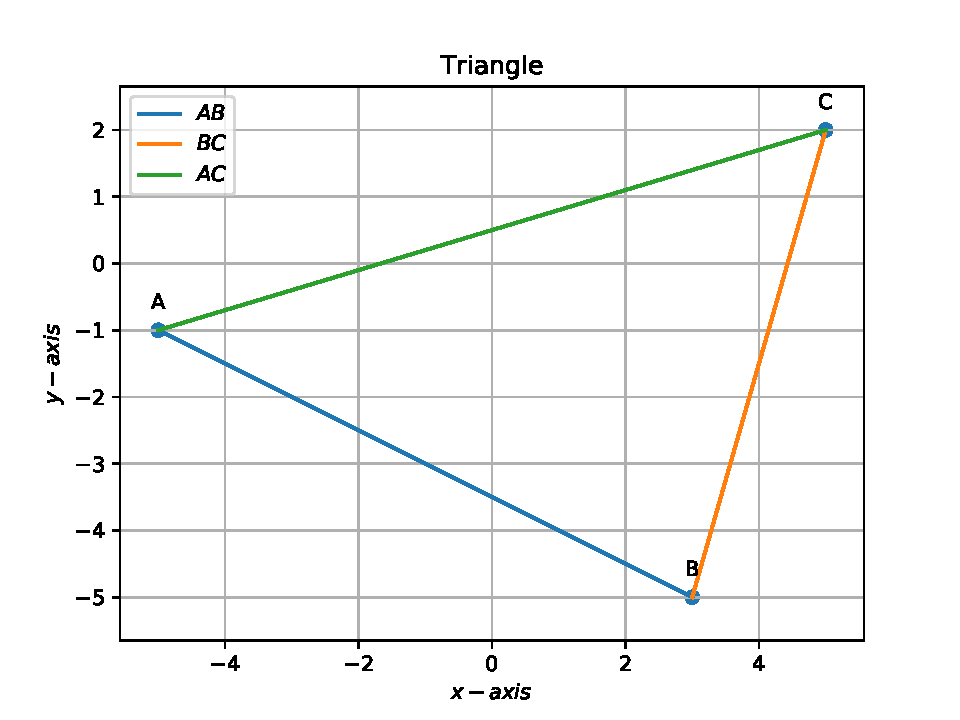
\includegraphics[width=\columnwidth]{./figs/problem1b.pdf}
	\end{center}
\caption{}
\label{fig:Fig2}
\end{figure}
\fi
\end{enumerate}




\item In each of the following, find the value of '$k$', for which the points are collinear.
\begin{enumerate}
\item $(7, –2), (5, 1), (3, k)$
\item $(8, 1), (k, – 4), (2, –5)$
\end{enumerate}
		\label{10/7/3/2}
\solution
%		\iffalse
\documentclass[journal,12pt,twocolumn]{IEEEtran}
\usepackage{graphicx}
\graphicspath{{./figs/}}{}
\usepackage{amsmath,amssymb,amsfonts,amsthm}
\newcommand{\myvec}[1]{\ensuremath{\begin{pmatrix}#1\end{pmatrix}}}
\providecommand{\norm}[1]{\lVert#1\rVert}
\usepackage{listings}
\usepackage{watermark}
\usepackage{titlesec}
\usepackage{caption}
\usepackage{enumitem}
\usepackage{extarrows}
\let\vec\mathbf
\lstset{
frame=single, 
breaklines=true,
columns=fullflexible
}
\thiswatermark{\centering \put(0,-105.0){
\includegraphics[scale=0.15]{/sdcard/IITH/vector/vector-3/figs/logo.png}} }
\title{\mytitle}
\title{
Assignment - Vector-3
}
\author{Surajit Sarkar}
\begin{document}
\maketitle
\tableofcontents
\bigskip
\section{\textbf{Problem}}
In each of the following, find the value of ’k’,\\ for which the points are collinear.
\begin{enumerate}[label=(\roman*)]
\item (7, –2), (5, 1), (3, k)
\item(8, 1), (k, –4), (2, –5)
\end{enumerate}
\section{\textbf{Solution}}
\fi
\begin{enumerate}
    \item Given
    \begin{align}
      \vec{A}=\myvec{7\\-2},\Vec{B}=\myvec{5\\1},\vec{C}=\myvec{3\\k}  
    \end{align}
    Then
    \begin{align}
        \myvec{\vec{A}-\vec{B}}&=\myvec{2\\-3}\\
        \myvec{\vec{A}-\vec{C}}&=\myvec{4\\2k}\
    \end{align}
    Forming the collinearity matrix
    \begin{align}
        \myvec{2&-3\\4&2k} \xleftrightarrow{R_1\rightarrow{R_1-1}}&\myvec{1&-2\\4&2k}\\
         \xleftrightarrow{R_1\rightarrow{R_1-1}}&\myvec{1&-2\\0&2k+8}\\
        k&=4
        \end{align}
    
    \item Given
     \begin{align}
      \vec{A}=\myvec{8\\1},\vec{B}=\myvec{k\\-4},\vec{C}=\myvec{2\\-5}  
    \end{align}
    Then
    \begin{align}
        \myvec{\vec{A}-\vec{B}}&=\myvec{-8k\\-5}\\
        \myvec{\vec{A}-\vec{C}}&=\myvec{6\\6}\
    \end{align}
    Forming the collinearity matrix
    \begin{align}
        \myvec{-8-k&-5\\6&6} \xleftrightarrow{R_1\rightarrow{R_1+8}}&\myvec{-k&3\\6&6}\\
        k&=3
        \end{align}
\end{enumerate}



\item Find the area of the triangle formed by joining the mid-points of the sides of the triangle whose vertices are $(0, –1), (2, 1) \text{ and } (0, 3)$. Find the ratio of this area to the area of the given triangle.

\item Find the area of the quadrilateral whose vertices, taken in order, are $(– 4, – 2), (– 3, – 5), (3, – 2)$  and $ (2, 3)$.

\item Verify that a median of a triangle divides it into two triangles of equal areas for $\triangle ABC$ whose vertices are $\vec{A}(4, -6), \vec{B}(3, 2), \text{ and } \vec{C}(5, 2)$. 

\item Find the area of region bounded by the triangle whose
	vertices are $(1, 0), (2, 2) \text{ and } (3, 1)$. 
\item Find the area of region bounded by the triangle whose vertices
	are $(– 1, 0), (1, 3) \text{ and } (3, 2)$. 

\item Find the area of the $\triangle ABC$, coordinates of whose vertices are $\vec{A}(2, 0), \vec{B}(4, 5), \text{ and } \vec{C}(6, 3)$.

\end{enumerate}


